\documentclass{article}

\usepackage{geometry}
\usepackage{amsmath}
\usepackage{graphicx, eso-pic}
\usepackage{listings}
\usepackage{hyperref}
\usepackage{multicol}
\usepackage{fancyhdr}
\pagestyle{fancy}
\fancyhf{}
\hypersetup{ colorlinks=true, linkcolor=black, filecolor=magenta, urlcolor=cyan}
\geometry{ a4paper, total={170mm,257mm}, top=40mm, right=20mm, bottom=20mm, left=20mm}
\setlength{\parindent}{0pt}
\setlength{\parskip}{0.3em}
\renewcommand{\headrulewidth}{0pt}
\AddToShipoutPictureBG{%
  \AtPageUpperLeft{%
    \raisebox{-\height}{
\includegraphics[width=\paperwidth, height=30mm]{../headerarkav.png}}
  }
}
\rfoot{\thepage}
\lfoot{Final Competitive Programming - Arkavidia 7.0}
\lstset{
    basicstyle=\ttfamily\small,
    columns=fixed,
    extendedchars=true,
    breaklines=true,
    tabsize=2,
    prebreak=\raisebox{0ex}[0ex][0ex]{\ensuremath{\hookleftarrow}},
    frame=none,
    showtabs=false,
    showspaces=false,
    showstringspaces=false,
    prebreak={},
    keywordstyle=\color[rgb]{0.627,0.126,0.941},
    commentstyle=\color[rgb]{0.133,0.545,0.133},
    stringstyle=\color[rgb]{01,0,0},
    captionpos=t,
    escapeinside={(\%}{\%)}
}

\begin{document}

\begin{center}
    \section*{K - Kalkulator} % ganti judul soal

    \begin{tabular}{ | c c | }
        \hline
        Batas Waktu  & 5s \\    % jangan lupa ganti time limit
        Batas Memori & 256MB \\  % jangan lupa ganti memory limit
        \hline
    \end{tabular}
\end{center}

\subsection*{Deskripsi}
Pascal memiliki sebuah kalkulator unik yang terdiri atas $M$ buah tombol, sehingga pada tombol ke-$i$ tertulis bilangan $A_{i}$, dan sebuah bilangan $N$ yang menandakan versi dari kalkulator tersebut. Setiap kali Pascal menekan tombol ke-$i$, bilangan pada layar kalkulator akan bertambah sebanyak $A_{i}$, kemudian dimodulo dengan $N$.
\begin{center}
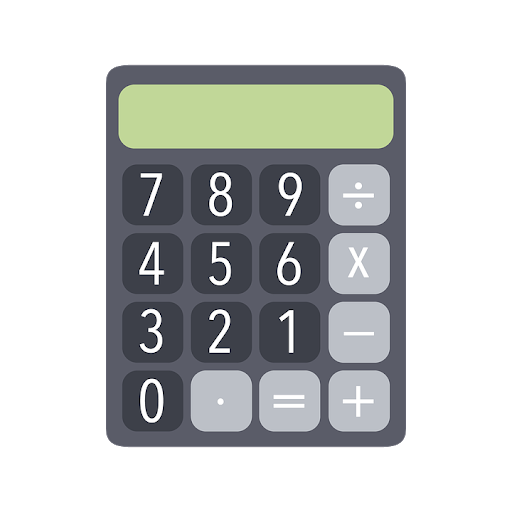
\includegraphics[scale=0.24]{kalkulator.png}
\end{center}
Pada awalnya, bilangan awal pada layar kalkulator bernilai 0. Pascal ingin menekan $R$ buah tombol satu per satu (tidak harus tombol berbeda) sehingga bilangan akhir pada layar kalkulator bernilai $X$, untuk setiap nilai $X$ dari $0$ hingga $N-1$, bantulah Pascal untuk menghitung banyaknya cara menekan tombol berbeda yang mungkin. Dua cara penekanan dikatakan berbeda apabila terdapat suatu bilangan $K$ sehingga tombol dengan urutan penekanan ke-$K$ pada cara penekanan pertama berbeda dengan tombol dengan urutan penekanan ke-$K$ pada cara penekanan kedua.

Karena bilangan dapat bernilai sangat besar, keluarkan jawaban dimodulo $998244353$.

\subsection*{Format Masukan}
Baris pertama berisi tiga buah bilangan bulat $N$ ($1 \le N \le 3 \cdot 10^4$), $M$ ($1 \le M \le 10^6$) dan $R$ ($1 \le R \le 10^{18}$) yang masing - masing menyatakan versi kalkulator milik Pascal, banyaknya tombol pada kalkulator milik Pascal dan banyaknya tombol yang ditekan Pascal.

Baris berikutnya berisi $M$ buah bilangan bulat $A_1, A_2, \dots, A_M$ ($1 \le A_i \le 10^9$ untuk setiap $i$ dengan $1 \leq i \leq M$) dipisahkan oleh spasi yang menyatakan bilangan-bilangan pada tombol-tombol kalkulator milik Pascal.

\subsection*{Format Keluaran}
Sebuah baris yang terdiri atas $N$ buah bilangan yang dipisahkan dengan spasi, dengan bilangan ke-$i$ menyatakan banyaknya cara Pascal menekan $R$ tombol satu per satu (tidak harus berbeda) sehingga bilangan akhir pada layar kalkulator adalah $i - 1$ dimodulo $998244353$.

\begin{multicols}{2}
\subsection*{Contoh Masukan 1}
\begin{lstlisting}
2 2 3
2 3
\end{lstlisting}
\columnbreak
\subsection*{Contoh Keluaran 1}
\begin{lstlisting}
4 4
\end{lstlisting}
\vfill
\null
\end{multicols}

\begin{multicols}{2}
\subsection*{Contoh Masukan 2}
\begin{lstlisting}
3 3 2
10 10 10
\end{lstlisting}
\columnbreak
\subsection*{Contoh Keluaran 2}
\begin{lstlisting}
0 0 9
\end{lstlisting}
\vfill
\null
\end{multicols}


\pagebreak
\subsection*{Penjelasan}
Pada kasus uji pertama,
\begin{itemize}
    \item Semua cara berbeda yang mungkin untuk membentuk angka 0 adalah:
    \begin{itemize}
        \item 2 2 2
        \item 2 3 3
        \item 3 2 3
        \item 3 3 2
    \end{itemize}
    
    \item Semua cara berbeda yang mungkin untuk membentuk angka 1 adalah:
    \begin{itemize}
        \item 3 2 2
        \item 2 3 2
        \item 2 2 3
        \item 3 3 3
    \end{itemize}
\end{itemize}
\end{document}